\documentclass[tikz]{standalone}
\usetikzlibrary{patterns}
\usetikzlibrary{arrows}
\usetikzlibrary{decorations.shapes,decorations.markings,decorations.pathreplacing}

\tikzset{
    set arrow inside/.code={\pgfqkeys{/tikz/arrow inside}{#1}},
    set arrow inside={end/.initial=>, opt/.initial=},
    /pgf/decoration/Mark/.style={
        mark/.expanded=at position #1 with
        {
            \noexpand\arrow[\pgfkeysvalueof{/tikz/arrow inside/opt}]{\pgfkeysvalueof{/tikz/arrow inside/end}}
        }
    },
    arrow inside/.style 2 args={
        set arrow inside={#1},
        postaction={
            decorate,decoration={
                markings,Mark/.list={#2}
            }
        }
    },
}

\begin{document}
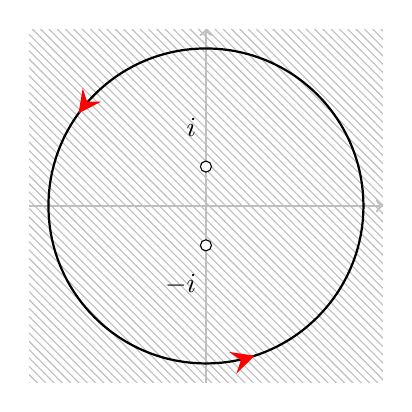
\begin{tikzpicture}
\draw[pattern=north west lines,pattern color=gray!50,draw=white] (-2.25,-2.25) -- (-2.25,2.25) -- (2.25,2.25) -- (2.25,-2.25) -- (-2.25,-2.25);
\draw[->,thick,color=gray!50] (-2.25,0) -- (2.25,0) ;%node[right];%{$\mathrm{Re}$};
\draw[->,thick,color=gray!50] (0,-2.25) -- (0,2.25) ;%node[above];%{$\mathrm{Im}$};
\draw[thick] (0,0) circle (2) [arrow inside={end=stealth,opt={red,scale=2}}{0.4,0.8}];
%\draw[thick] (2,0) arc (0:180:2);
%\draw[thick] (-2,0) --(2,0) [arrow inside={end=stealth,opt={red,scale=2}}{0.3}];
%\draw (-2,0) node[below]{$-R$};
%\draw (2,0) node[below]{$R$};
%\draw[yshift=0.25cm] (0,2) node[above,left]{$iR$};
%\draw[thick] (-2,0) -- (2,0);
\draw[fill=white] (0,0.5) circle(2pt);
\draw (0,1) node[left]{$i$};
\draw (0,-1) node[left]{$-i$};
\draw[fill=white] (0,-0.5) circle(2pt);
\end{tikzpicture}
\end{document}